\documentclass[12pt]{report}
\usepackage[utf8]{inputenc}
\usepackage[russian]{babel}
%\usepackage[14pt]{extsizes}
\usepackage{listings}
\usepackage{graphicx}
\usepackage{amsmath,amsfonts,amssymb,amsthm,mathtools} 
\usepackage{pgfplots}
\usepackage{filecontents}
\usepackage{indentfirst}
\usepackage{eucal}
\usepackage{amsmath}
\usepackage{enumitem}
\usepackage{fixltx2e}
\usepackage{float}

\frenchspacing

\usepackage{indentfirst} % Красная строка


%\usetikzlibrary{datavisualization}
%\usetikzlibrary{datavisualization.formats.functions}

\usepackage{amsmath}


% Для листинга кода:
\lstset{ %
language=caml,                 % выбор языка для подсветки (здесь это С)
basicstyle=\small\sffamily, % размер и начертание шрифта для подсветки кода
numbers=left,               % где поставить нумерацию строк (слева\справа)
numberstyle=\tiny,           % размер шрифта для номеров строк
stepnumber=1,                   % размер шага между двумя номерами строк
numbersep=5pt,                % как далеко отстоят номера строк от подсвечиваемого кода
showspaces=false,            % показывать или нет пробелы специальными отступами
showstringspaces=false,      % показывать или нет пробелы в строках
showtabs=false,             % показывать или нет табуляцию в строках
frame=single,              % рисовать рамку вокруг кода
tabsize=2,                 % размер табуляции по умолчанию равен 2 пробелам
captionpos=t,              % позиция заголовка вверху [t] или внизу [b] 
breaklines=true,           % автоматически переносить строки (да\нет)
breakatwhitespace=false, % переносить строки только если есть пробел
escapeinside={\#*}{*)}   % если нужно добавить комментарии в коде
}

\usepackage[left=2cm,right=2cm, top=2cm,bottom=2cm,bindingoffset=0cm]{geometry}


% plot
\usepackage{pgfplots}
\usepackage{filecontents}
\usetikzlibrary{datavisualization}
\usetikzlibrary{datavisualization.formats.functions}

\graphicspath{ {img/} }


\usepackage{subcaption}

\captionsetup{labelsep=endash}
\captionsetup[figure]{name={Рисунок}}


\begin{document}
	\begin{titlepage}
		\thispagestyle{empty}
		
		\noindent
		\begin{minipage}{0.15\textwidth}
			
\includegraphics[width=\linewidth]{main_logo}
		\end{minipage}
		\noindent
		\begin{minipage}{0.9\textwidth}
			\centering
			\textbf{Министерство науки и высшего образования Российской Федерации}\\
			\textbf{Федеральное государственное бюджетное образовательное учреждение высшего образования}\\
			\textbf{«Московский государственный технический университет имени Н.Э.~Баумана}\\
			\textbf{(национальный исследовательский университет)»}\\
			\textbf{(МГТУ им. Н.Э.~Баумана)}
		\end{minipage}
		
		\noindent
		\rule{18cm}{3pt} %пустая строка
		\newline\newline %пустая строка
		\noindent ФАКУЛЬТЕТ $\underline{\text{«Информатика и системы управления»}}$ \newline\newline
		\noindent КАФЕДРА $\underline{\text{«Программное обеспечение ЭВМ и информационные технологии»}}$\newline\newline\newline\newline\newline
		
		
		\begin{center}
			\noindent\begin{minipage}{1.3\textwidth}\centering
				\Large\textbf{  Отчёт о лабораторной работе №1}\newline
				\textbf{по дисциплине "Анализ алгоритмов"}\newline
				\textbf{на тему "Расстояния Левенштейна и}\newline
				\textbf{Дамерау-Левенштейна"}\newline\newline
			\end{minipage}
		\end{center}
		
		\noindent\textbf{Студент} $\underline{\text{Коняев Е.А}}$\newline\newline
		\noindent\textbf{Группа} $\underline{\text{ИУ7-53Б}}$\newline\newline
		\noindent\textbf{Преподаватели} $\underline{\text{Волкова Л.Л., Строганов Ю.В.}}$\newline\newline
		\noindent\textbf{Дата сдачи отчета}$\underline{\text{~~~~~~~~~~~~~~~~~~~~~~~~~~~}}$\newline\newline
		\noindent\textbf{Оценка (баллы)} $\underline{\text{~~~~~~~~~~~~~~~~~~~~~~~~~~~}}$\newline\newline\newline
		
		\begin{center}
			\vfill
			Москва~---~\the\year~г.
		\end{center}
	\end{titlepage}
	
	\setcounter{page}{2}
	\tableofcontents
	
	\newpage
	\chapter*{Введение}
	
	\addcontentsline{toc}{chapter}{Введение}
	
	
Обработка строк является важной частью в сфере программирования и алгоритмики, так как она используется при решении многих важных задач, например:

\begin{enumerate}
	\item[1)] поиска слова в тексте;
	\item[2)] проверки текстов на орфографию;
	\item[3)] сравнения файлов.
\end{enumerate}

Среди всех алгоритмов работы со строками одними из важнейших являются методы их сравнения, некоторые из которых будут рассмотрены в данной лабораторной работе.

	
	\chapter{Аналитическая часть}
	
	\section{Цель и задачи}
	
	Целью данной работой является изучение метода динамического программирования на основании определения редакционных расстояний с помощью алгоритмов Левенштейна и Дамерау-Левенштейна. Для достижения поставленной цели требуется решить следующие задачи:
	
	\begin{enumerate}
		\item[1)] изучить и рассмотреть алгоритмы Левенштейна и Дамерау-Левенштейна;
		\item[2)] построить блок-схемы данных алгоритмов;
		\item[3)] реализовать каждый из алгоритмов;
		\item[4)] оценить их ресурсозатратность по памяти;
		\item[5)] экспериментально оценить временные характеристики алгоритмов;
		\item[6)] сделать вывод на основании проделанной работы.
	\end{enumerate}
	
	
	\section{Итерационный алгоритм нахождения расстояния Левенштейна}
	
	Расстояние Левенштейна является мерой сходства между двумя строками. Пусть исходная строка $S_{1}$, а целевая строка $S_{2}$. Тогда рассматриваемое расстояние -- это количество \textbf{удалений} (Delete), \textbf{вставок} (Insert) или \textbf{замен} (Replace), которые необходимо совершить для того, чтобы преобразовать $S_{1}$ в $S_{2}$. Чем больше расстояние Левенштейна, тем больше отличаются строки.
	
	Принято для вышеописанных операций вводить штраф равный единице. Само же расстояние Левенштейна вычисляется по руккурентной формуле (формуле, использующей значения предыдущих членов ряда для вычесления последующих):
	
	\begin{equation}
	\label{dlformula}
	D(i, j) = \begin{cases}
		
		0, &\text{i = 0, j = 0}\\
		i, &\text{j = 0, i > 0}\\
		j, &\text{i = 0, j > 0}\\
		\min \lbrace \\
		\qquad D(i, j-1) + 1,\\
		\qquad D(i-1, j) + 1, &\text{i > 0, j > 0}\\
		\qquad D(i-1, j-1) + \begin{cases}
                        		0, &\text{если $S_{i}$ = $S_{j}$,}\\
                        		1, &\text{иначе}
                        	\end{cases}\\
		\rbrace,
	\end{cases}
	\end{equation}
	
	В итерационном алгоритме нахождения расстояния Левенштейна используется формула (\ref{dlformula}).
	
	
	\section{Итерационный алгоритм нахождения расстояния Дамерау-Левенштейна}
	
	Алгоритм нахождения расстояния Дамерау-Левенштейна отличается от предыдущего тем, что в нем, помимо операций удаления, вставки, замены, в нем присутствует еще и \textbf{транспозиция двух символов} (Match). Данную операцию Домерау предложил из сооброжений, что перестановка соседних символов местами -- одна из самых частых ошибок при наборе рукописного текста. Штраф транспозиции двух символов так же равен единице.
	
	Таким образом, в реккурентной формуле (\ref{dlformula}) необходимо добавить еще одно определение минимума, в случае, когда возможна перестановка двух сосетдних симоволов:
	
	\begin{equation}
	\label{ddlformula}
	D(i, j) = \begin{cases}
		
		0, &\text{i = 0, j = 0,}\\
		i, &\text{j = 0, i > 0,}\\
		j, &\text{i = 0, j > 0,}\\
		
		\min \lbrace \\
		\qquad D(i, j-1) + 1,&\text{i > 0, j > 0,}\\
		\qquad D(i-1, j) + 1,&\text{$S_{i}$ = $S_{j-1}$,}\\
		\qquad D(i-2, j-2) + 1,&\text{$S_{i-1}$ = $S_{j}$,}\\
		\qquad D(i-1, j-1) + \begin{cases}
                        		0, &\text{если $S_{i}$ = $S_{j}$,}\\
                        		1, &\text{иначе}
                        	\end{cases}\\
		\rbrace,\\
		
		\min \lbrace \\
		\qquad D(i, j-1) + 1,\\
		\qquad D(i-1, j) + 1,&\text{иначе}\\
		\qquad D(i-1, j-1) + \begin{cases}
                        		0, &\text{если $S_{i}$ = $S_{j}$,}\\
                        		1, &\text{иначе}
                        	\end{cases}\\
		\rbrace
	\end{cases}
	\end{equation}
	
	Именно на формуле (\ref{ddlformula}) основан итерационный алгоритм нахождения расстояния Дамерау-Левенштейна.
	
	\section{Рекурсивный алгоритм нахождения расстояния Дамерау-Левенштейна}
	
	Рекурсивный алгоритм нахождения расстояния Дамерау-Левенштейна отличается от его итерационной разновидности тем, что в нем не используется матрица для хранения предыдущих значений, необходимых для подсчета последующих. Вместо этого данные значения вычисляются каждый раз рекурсивно. 
	
	\section{Рекурсивный алгоритм нахождения расстояния Дамерау-Левенштейна с использованием кеша}
	Данный алгоритм является оптимизацией рекурсивного алгоритма нахождения расстояния Дамерау-Левенштейна. Оптимизация заключается в использовании кеша, который представляется собой матрицу, в которую записываются значения, вычисленные на шагах рекурсии. Таким образом, при необходимости вычисления какого-либо нового значения по реккурентной формуле, величины, необходимые для этого не находятся каждый раз: сначала проверяется, было ли вычислено данное значения ранее, и только лишь в случае, если этого не происходило, выполняются рекурсивные вычисления для его получения.
	
	
	\section*{Вывод}
	
	В данном разделе были рассмотрены алгоритмы Левенштейна и Дамерау-Левенштейна, позволяющие находить редакционные расстояния для строк.
	
	\clearpage
	
	\chapter{Конструкторская часть}
	
	В данном разделе будут представлены описание типов данных, теоретическая оценка затрат алгоритмов по памяти и схемы алгоритмов. 
	
	\section{Описание типов данных}
	
	Для реализации алгоритмов Левенштейна и Дамерау-Левенштейна были использованы типы данных:

	\begin{enumerate}
	\item[1)] две строки, каждая из которых является массивом типа $char$;
	\item[2)] длины строк -- тип $int$;
	\item[3)] структура матрицы, которая состоит из ее размерностей (2 числа типа $int$) и двумерного массива элементов типа $int$.
	\end{enumerate}
	
	\section{Оценка затрат алгоритмов по памяти}
	
	Затраты по памяти для алгоритма поиска расстояния Левенштайна (итерационного):

	\begin{enumerate}
	\item[1)] длины строк n, m -- $2 \cdot sizeof(int)$;
	\item[2)] матрица -- $(n + 1) \cdot (m + 1) \cdot sizeof(int) + 2 \cdot sizeof(int)$;
	\item[3)] строки -- $(n + m + 2) \cdot sizeof(char)$;
	\item[4)] дополнительные переменные (i, j, res, offset) -- $4 \cdot sizeof(int)$; 
	\item[5)] адрес возврата.
	\end{enumerate}
	
	Суммарные затраты по памяти:
	
	$(n + 1) \cdot (m + 1) \cdot sizeof(int) + 7 \cdot sizeof(int) + (n + m + 2) \cdot sizeof(char)$\newline\newline\newline\newline\newline\newline\newline
	
	Затраты по памяти для алгоритма поиска расстояния Дамерау-Левенштейна (итерационного):
	
	\begin{enumerate}
	\item[1)] длины строк n, m -- $2 \cdot sizeof(int)$;
	\item[2)] матрица -- $(n + 1) \cdot (m + 1) \cdot sizeof(int) + 2 \cdot sizeof(int)$;
	\item[3)] строки -- $(n + m + 2) \cdot sizeof(char)$;
	\item[4)] дополнительные переменные (i, j, res, offset) -- $4 \cdot sizeof(int)$; 
	\item[5)] адрес возврата.
	\end{enumerate}
	
	Суммарные затраты по памяти:
	
	$(n + 1) \cdot (m + 1) \cdot sizeof(int) + 7 \cdot sizeof(int) + (n + m + 2) \cdot sizeof(char)$\newline
	
	Затраты по памяти для алгоритма поиска расстояния Дамерау-Левенштейна (рекурсивного) для одного вызова:
	
	\begin{enumerate}
	\item[1)] длины строк n, m -- $2 \cdot sizeof(int)$;
	\item[2)] строки -- $(n + m + 2) \cdot sizeof(char)$;
	\item[3)] дополнительные переменные (res, offset) -- $2 \cdot sizeof(int)$; 
	\item[4)] адрес возврата.
	\end{enumerate}
	
	Суммарные затраты по памяти (R -- количество вызовов рекурсии):
	
	$(4 \cdot sizeof(int) + (n + m + 2) \cdot sizeof(char)) \cdot R$\newline
	
	Затраты по памяти для алгоритм поиска расстояния Дамерау-Левенштейна (рекурсивного с кешем) для одного вызова:
	
	\begin{enumerate}
	\item[1)] длины строк n, m -- $2 \cdot sizeof(int)$;
	\item[2)] строки -- $(n + m + 2) \cdot sizeof(char)$;
	\item[3)] дополнительные переменные (res, offset) -- $2 \cdot sizeof(int)$; 
	\item[4)] матрица -- $(n + 1) \cdot (m + 1) \cdot sizeof(int) + 2 \cdot sizeof(int)$;
	\item[5)] адрес возврата.
	\end{enumerate}
	
	Суммарные затраты по памяти (R -- количество вызовов рекурсии):
	
	$(6 \cdot sizeof(int) + (n + m + 2) \cdot sizeof(char)) \cdot R + (n + 1) \cdot (m + 1) \cdot sizeof(int)$\newline
	
	\section{Описания алгоритмов}
	
	На рисунках ниже показаны схемы алгоритмов Левенштейна и Дамерау-Левенштейна.
	
	\begin{figure}[H]
		\centering
		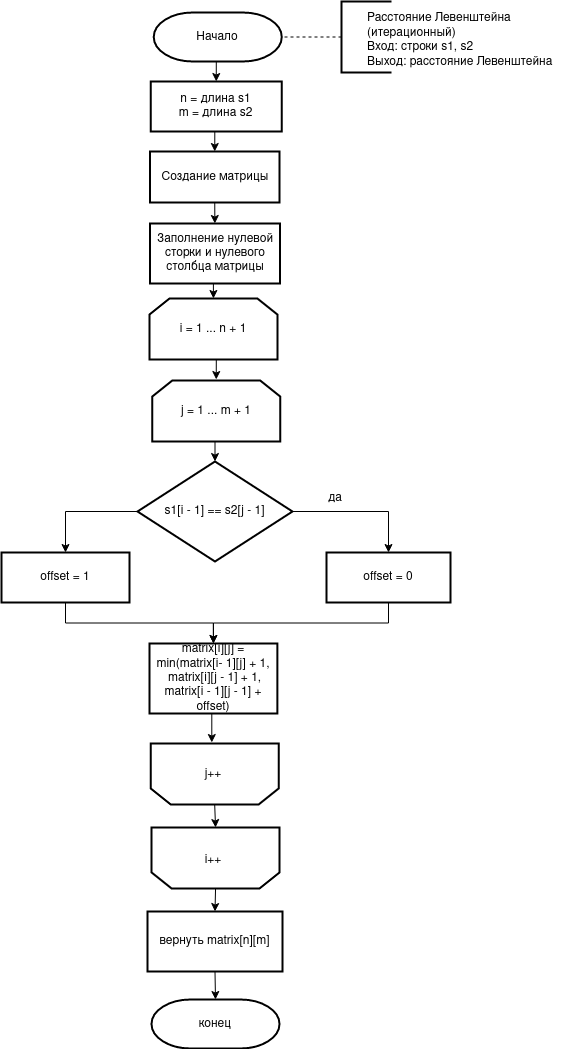
\includegraphics[width=0.6\linewidth]{Lev}
		\caption{Схема итерационного алгоритма поиска расстояния Левенштейна}
		\label{fig:schema_bucket_1}
	\end{figure}
	
	\begin{figure}[H]
		\centering
		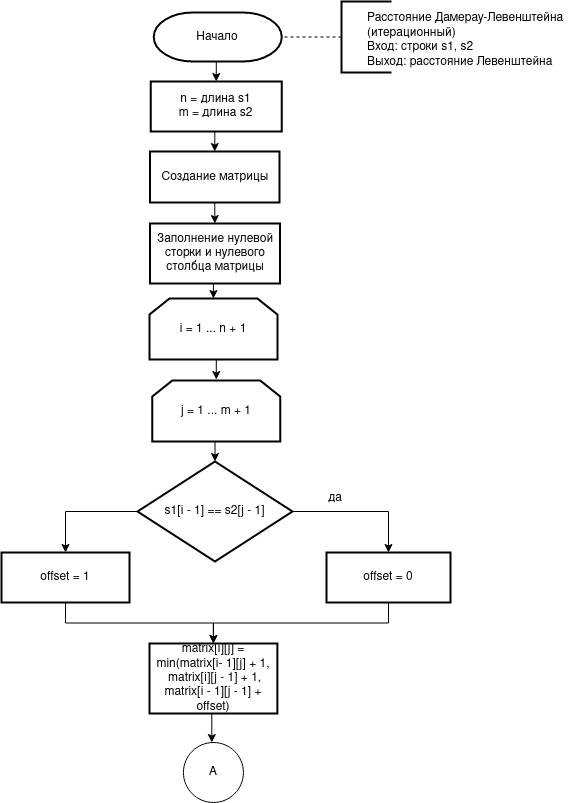
\includegraphics[width=0.8\linewidth]{DamLev_1}
		\caption{Схема итерационного алгоритма поиска расстояния Дамерау-Левенштейна, ч.1}
		\label{fig:schema_bucket_2}
	\end{figure}
	
	\begin{figure}[H]
		\centering
		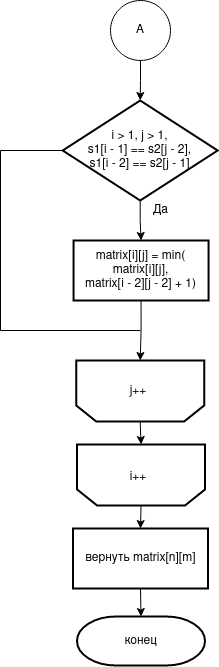
\includegraphics{DamLev_2}
		\caption{Схема итерационного алгоритма поиска расстояния Дамерау-Левенштейна, ч.2}
		\label{fig:schema_bucket_3}
	\end{figure}
	
	\begin{figure}[H]
		\centering
		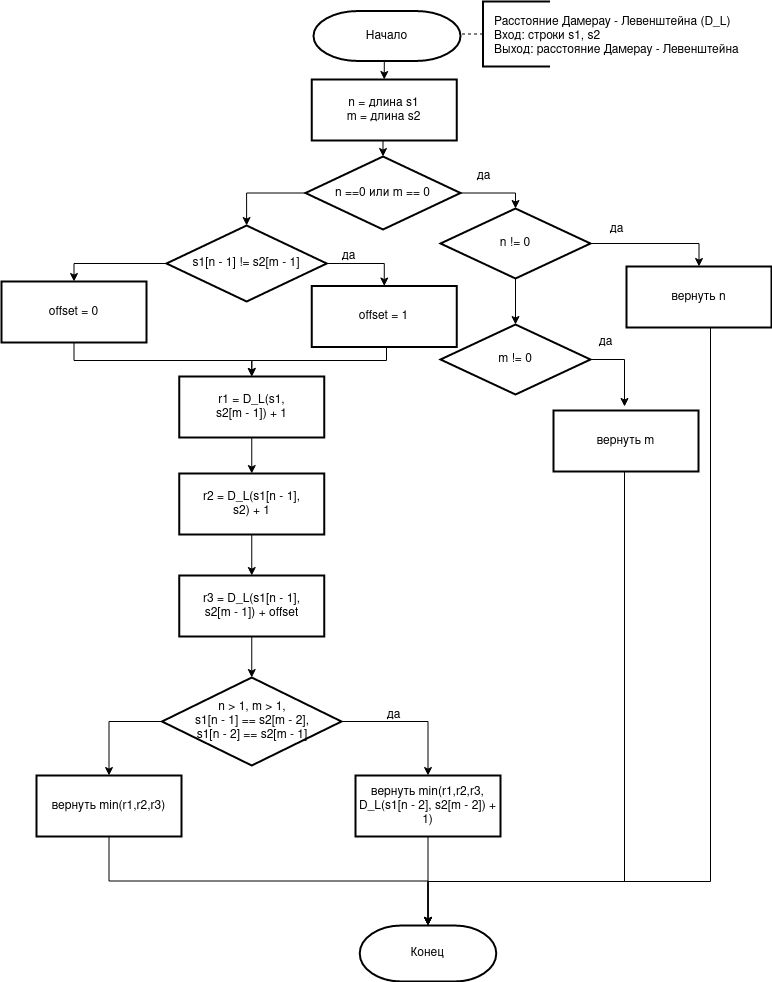
\includegraphics[width=0.8\linewidth]{DamLevRec}
		\caption{Схема рекурсивного алгоритма поиска расстояния Дамерау-Левенштейна}
		\label{fig:schema_selection}
	\end{figure}
	
	\begin{figure}[H]
		\centering
		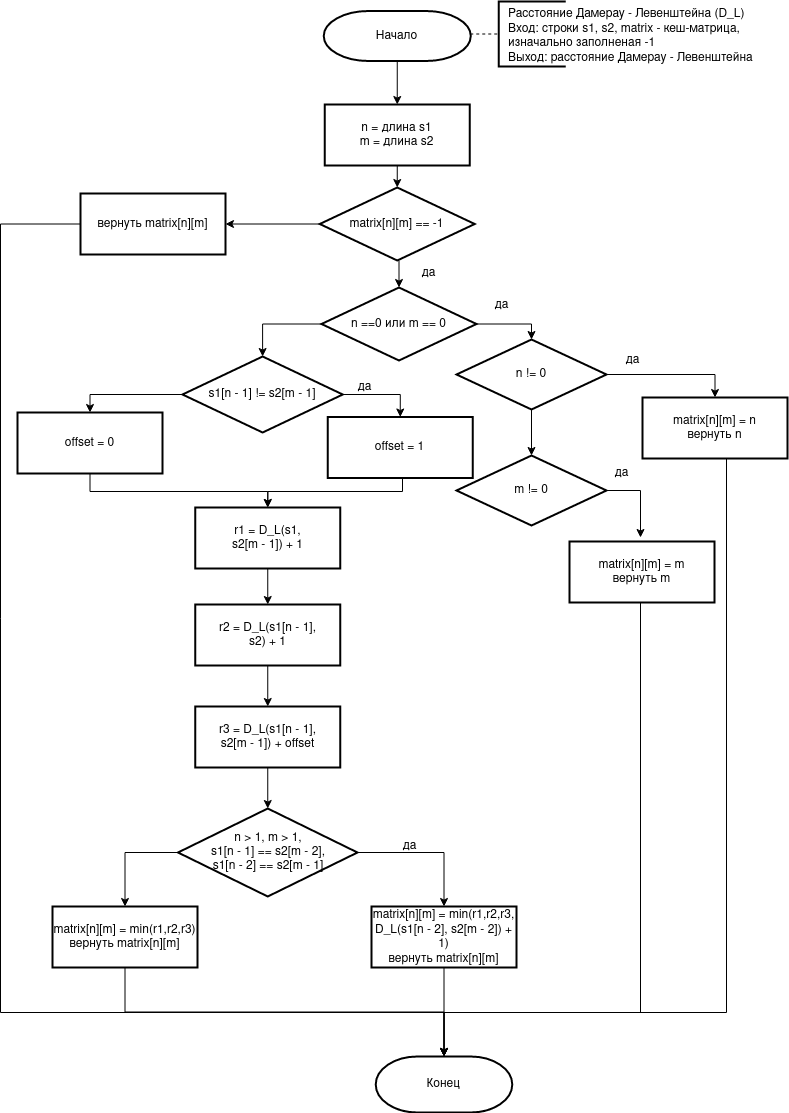
\includegraphics[width=0.8\linewidth]{DamLevRecHash}
		\caption{Схема рекурсивного алгоритма поиска расстояния Дамерау-Левенштейна с кешем}
		\label{fig:schema_selection}
	\end{figure}
	
	\section*{Вывод}
	
	В данном разделе были представлены описания алгоритмов Левенштейна и Дамерау-Левенштейна, а так же проведена теоретическая оценка затрат алгортмов по памяти, которая показала, что рекурсивные алгоритмы менее затратны по памяти.
	
	\chapter{Технологическая часть}
	
	В данном разделе приведены требования к ПО, обоснования выбора языка программирования, среды разработки, приведен способ замера времени выполнения, а также приведены листинги кода.
	
	\section{Требования к ПО}
	
	В программе должна присутствовать возможность:
	
	\begin{enumerate}
		\item[1)] ввода исходных строк, для которых будет находиться расстояния Левенштейна и Дамерау-Левенштейна;
		\item[2)] поиска искомого расстояния для введеных строк с помощью одного из четырех рассматриваемых алгоритмов;
		\item[3)] замера процессорного времени выполнения реализаций алгоритмов поиска расстояний Левенштейна и Дамерау-Левенштейна.
	\end{enumerate}
	
	\section{Выбор языка программирования и среды разработки}
	
	Для реализации трех алгоритмов сортировок был выбор язык С, так как я уже имею опыт разработки на данном языке программирования.

	Средой разработки был выбран СLion. Данный выбор обусловлен тем, что данная среда предоставляет возможность разработки приложений под C/C++ и имеет инструменты для отладки кода. 
	
	\section{Выбор библиотеки и способа для замера времени}
		Для замера времени выполнения сортировок использовалась стандартная функция библиотеки <time.h> языка С~---~clock(), которая замеряет процессорное время. Если измерить время перед началом выполнения алгоритма, и после его окончания, то можно получить время выполнения функции. Реализация данной функции приведена в [1].
		
		Поскольку все процессорное время не отдается какой-либо одной задаче (в связи с явлением вытеснения процессов из ядра, квантование процессорного времени), то требуется усреднить результаты вычислений: замерить совокупное время выполнения реализации алгоритма N раз и вычислить среднее время выполнения.
		
	\section{Реализации алгоритмов}
	
	В листингах \ref{lev},\ref{damlev},\ref{damlevrec},\ref{damlevrechash} приведены реализации алгоритмов поиска расстояний Левенштейна (итерационный), Дамера-Левенштейна (итерационный), Дамерау-Левенштейна (рекурсивный), Дамерау-Левенштейна (рекурсивный с кешем) соответсвенно.
	
	\begin{lstlisting}[label=lev,caption=Листинг итерационного алгоритма поиска расстояния Левенштейна,language=C]
		int dist_lev(char *str_1, char *str_2)
		{
		    matrix_t *d = create_matrix(strlen(str_1) + 1, strlen(str_2) + 1);

		    d->elements[0][0] = 0;
		    for (size_t i = 1; i < d->rows; ++i)
			d->elements[i][0] = i;
		    for (size_t i = 1; i < d->cols; ++i)
			d->elements[0][i] = i;

		    for (size_t i = 1; i < d->rows; ++i)
			for (size_t j = 1; j < d->cols; ++j) {
			    int offset = str_1[i - 1] == str_2[j - 1] ? 0 : 1;
			    d->elements[i][j] = get_min(d->elements[i][j - 1] + 1,
				                        get_min(d->elements[i - 1][j] + 1,
				                                d->elements[i - 1][j - 1] + offset));
			}

		    int res = d->elements[d->rows - 1][d->cols - 1];
		    free_matrix(d);

		    return res;
		}
	\end{lstlisting}

	
	\begin{lstlisting}[label=damlev,caption=Листинг итерационного алгоритма поиска расстояния Дамерау-Левенштейна,language=C]
		int dist_dameray_lev(char *str_1, char *str_2)
		{
		    matrix_t *d = create_matrix(strlen(str_1) + 1, strlen(str_2) + 1);

		    d->elements[0][0] = 0;
		    for (size_t i = 1; i < d->rows; ++i)
			d->elements[i][0] = i;
		    for (size_t i = 1; i < d->cols; ++i)
			d->elements[0][i] = i;

		    for (size_t i = 1; i < d->rows; ++i)
			for (size_t j = 1; j < d->cols; ++j) {
			    int offset = str_1[i - 1] == str_2[j - 1] ? 0 : 1;
			    d->elements[i][j] = get_min(d->elements[i][j - 1] + 1,
				                        get_min(d->elements[i - 1][j] + 1,
				                                d->elements[i - 1][j - 1] + offset));
			    if (j > 1 && i > 1 && str_1[i - 1] == str_2[j - 2] && str_1[i - 2] == str_2[j - 1])
				d->elements[i][j] = get_min(d->elements[i][j], d->elements[i - 2][j - 2] + 1);
			}

		    int res = d->elements[d->rows - 1][d->cols - 1];
		    free_matrix(d);

		    return res;
		}
	\end{lstlisting}
	
	\bigbreak

	\begin{lstlisting}[label=damlevrec,caption=Листинг рекурсивного алгоритма поиска расстояния Дамерау-Левенштейна,language=C]
		int dist_dameray_lev_rec(char *str_1, char *str_2, int len_1, int len_2)
		{
		    if (len_1 == 0)
			return len_2;
		    if (len_2 == 0)
			return len_1;

		    int offset = str_1[len_1 - 1] == str_2[len_2 - 1] ? 0 : 1;
		    int res = get_min(dist_dameray_lev_rec(str_1, str_2, len_1 - 1, len_2) + 1,
				     get_min(dist_dameray_lev_rec(str_1, str_2, len_1, len_2 - 1) + 1,
				             dist_dameray_lev_rec(str_1, str_2, len_1 - 1, len_2 - 1) + offset));
		    if (len_1 > 1 && len_2 > 1 && str_1[len_1 - 1] == str_2[len_2 - 2] && str_1[len_1 - 2] == str_2[len_2 - 1])
			res = get_min(res, dist_dameray_lev_rec(str_1, str_2, len_1 - 2, len_2 - 2) + 1);

		    return res;
		}
	\end{lstlisting}
	
	\begin{lstlisting}[label=damlevrechash,caption=Листинг рекурсивного алгоритма поиска расстояния Дамерау-Левенштейна с кешем,language=C]	
		int dist_dameray_lev_rec_hash_call(char *str_1, char *str_2, int len_1, int len_2, matrix_t *mat)
		{
		    if (len_1 == 0)
			return (mat->elements)[len_1][len_2] = len_2;
		    if (len_2 == 0)
			return (mat->elements)[len_1][len_2] = len_1;

		    if (mat->elements[len_1 - 1][len_2] == -1)
			dist_dameray_lev_rec_hash_call(str_1, str_2, len_1 - 1, len_2, mat);
		    if (mat->elements[len_1][len_2 - 1] == -1)
			dist_dameray_lev_rec_hash_call(str_1, str_2, len_1, len_2 - 1, mat);
		    if (mat->elements[len_1 - 1][len_2 - 1] == -1)
			dist_dameray_lev_rec_hash_call(str_1, str_2, len_1 - 1, len_2 - 1, mat);

		    int offset = str_1[len_1 - 1] == str_2[len_2 - 1] ? 0 : 1;
		    mat->elements[len_1][len_2] = get_min(mat->elements[len_1][len_2 - 1] + 1,
				                get_min(mat->elements[len_1 - 1][len_2] + 1,
				                        mat->elements[len_1 - 1][len_2 - 1] + offset));
		    if (len_1 > 1 && len_2 > 1 && str_1[len_1 - 1] == str_2[len_2 - 2] && str_1[len_1 - 2] == str_2[len_2 - 1]) {
			if (mat->elements[len_1 - 2][len_2 - 2] == -1)
			    dist_dameray_lev_rec_hash_call(str_1, str_2, len_1 - 2, len_2 - 2, mat);
			mat->elements[len_1][len_2] = get_min(mat->elements[len_1][len_2], mat->elements[len_1 - 2][len_2 - 2] + 1);
		    }

		    return mat->elements[len_1][len_2];
		}

		int dist_dameray_lev_rec_hash(char *str_1, char *str_2)
		{
		    matrix_t *d = create_matrix(strlen(str_1) + 1, strlen(str_2) + 1);
		    clear_matrix_elems(d);

		    int res = dist_dameray_lev_rec_hash_call(str_1, str_2, strlen(str_1), strlen(str_2), d);
		    free_matrix(d);

		    return res;
		}
	\end{lstlisting}

	\section{Тестирование алгоритмов}

	В таблице~\ref{tbl:t1111111} приведены тесты для функций, реализующих алгоритмы поиска расстояний Левенштейна и Дамерау-Левенштейна. Все тесты пройдены успешно.\newline\newline
	
	\begin{table} [H]
		\caption{Тестирование функций алгоритмов Левинштейна и Дамерау-Левенштейна на разных входных строках}
		\center
		\label{table:t1111111}
			\begin{tabular}{|c | c | c | c | c|}
				
				\hline
				Первая строка & Вторая строка & Результат (Лев.) & Результат (Дам.-Лев.) \\ 
				\hline
				"пустая строка" & "пустая строка" & $0$ & $0$\\\hline
				$fit$  & "пустая строка" & $3$ & $3$\\\hline
				$fit$  & $fit$  & $0$ & $0$\\\hline
				$fit$  & $fiting$  & $3$ & $3$\\\hline
				$class$ & $calss$ & $2$ & $1$\\\hline
				
			\end{tabular}
	\end{table}


	\section*{Вывод}
	
	В данном разделе были разработаны исходные коды алгоритмов поиска расстояний Левенштейна и Дамерау-Левенштейна.
	
	\chapter{Экспериментальная часть}
	
	\section{Технические характеристики}
	
	Ниже приведены технические характеристики устройства, на котором было проведено тестирование ПО:
	
	\begin{enumerate}
		\item[1)] операционная система Windows-10, 64-bit;
		\item[2)] оперативная память 16 ГБ;
		\item[3)] процессор Intel(R) Core(TM) i7-8565U CPU @ 1.80 Ггц, 4 ядра, 8 логических процессоров.
	\end{enumerate}
	
	\section{Замеры времени}
	
	Введем обозначения: Lev -- итерационный алгоритм поиска расстояния Левенштейна, DamLev -- итерационный алгоритм поиска расстояния Дамерау-Левенштейна, DamLevRec -- рекурсивный алгоритм поиска расстояния Дамерау-Левенштейна, DamLevRecHash -- итерационный алгоритм поиска расстояния Дамерау-Левенштейна с кешем.
	
	В таблице \ref{table:t1} приведены результаты замеров времени алгоритмов для входных строк разной длины.
	
	\begin{table} [H]
		\caption{Таблица замера времени выполнения алгоритмов на строках, имеющих разные длины}
		\center
		\label{table:t1}
			\begin{tabular}{|c | c | c | c | c|}
				
				\hline
				
				Длина стоки & Lev & DamLev & DamLevRec &  DamLevRecHash \\ [0.5ex]
				
				\hline
				
				1 & 0.2 & 0.16 & 0.14 & 0.32 \\ 
				
				\hline 
				
				2 & 0.3 & 0.32 & 0.24 & 0.62 \\ 
				
				\hline 
				
				3 & 0.56 & 0.68 & 1.12 & 1.0 \\ 
				
				\hline 
				
				4 & 0.76 & 1.0 & 4.26 & 1.3 \\ 
				
				\hline 
				
				5 & 1.02 & 1.3 & 21.7 & 1.72 \\ 
				
				\hline 
				
				6 & 1.05 & 1.6 & 127.28 & 2.18 \\ 
				
				\hline 
				
				7 & 1.1 & 2.0 & 567.96 & 2.3 \\ 
				
				\hline 
				
				8 & 1.24 & 2.3 & 3170.12 & 3.08 \\ 
				
				\hline 
				
				9 & 1.42 & 2.3 & 18337.36 & 3.64\\ 
				
				\hline 
				
				10 & 1.94 & 2.38 & 102172.82 & 4.2\\ 
				
				\hline 
			\end{tabular}
	\end{table}

	Зависимость времени работы алгоритмов нахождения расстояния Левенштейна и Дамерау-Левенштейна от длины входных строк представлена на рис. \ref{ris1}.

	\begin{center}
		\begin{figure}[H]
		\center
		\begin{tikzpicture}
				\begin{axis} [
					legend pos = north west,
					grid = major,
					xmin = 0,
					ymin = 0, 
					xmax = 10,
					ymax = 103000,
					xlabel = $\text{длина входных строк}$,
					ylabel = $\text{время (мс)}$
					]
					\legend{ 
						$Lev$, 
						$DamLev$,
						$DamLevRec$,
						$DamLevRecHash$
					};
					\addplot coordinates {
						(1,0.2) (2,0.3) (3,0.56) (4,0.76) (5,1.02) (6,1.05) (7,1.10) (8,1.24) (9,1.42) (10,1.94)
					};
					\addplot coordinates {
						(1,0.16) (2,0.32) (3,0.68) (4,1.0) (5,1.3) (6,1.6) (7,2.0) (8,2.3) (9,2.3) (10,2.38)
					};
					\addplot coordinates {
						(1,0.14) (2,0.24) (3,1.12) (4,4.26) (5,21.7) (6,127.28) (7,567.96) (8,3170.12) (9,18337.36) (10,102172)
					};
					\addplot coordinates {
						(1,0.32) (2,0.62) (3,1.0) (4,1.3) (5,1.72) (6,2.18) (7,2.3) (8,3.08) (9,3.64) (10,4.2)
					};
				\end{axis}
		\end{tikzpicture}
		\caption{Зависимость времени от длины входных строк}
		\label{ris1}
		\end{figure}
	\end{center}
	
	
	Зависимость времени работы итерационных алгоритмов нахождения расстояния Левенштейна и Дамерау-Левенштейна от длины входных строк представлена на рис. \ref{ris2}.


	\begin{center}
		\begin{figure}[H]
		\center
		\begin{tikzpicture}
			\begin{axis} [
				legend pos = north west,
				grid = major,
				xmin = 0,
				ymin = 0, 
				xmax = 10,
				ymax = 2.5,
				xlabel = $\text{длина входных строк}$,
				ylabel = $\text{время (мс)}$
				]
				\legend{ 
					$Lev$, 
					$DamLev$,
				};
				\addplot coordinates {
					(1,0.2) (2,0.3) (3,0.56) (4,0.76) (5,1.02) (6,1.05) (7,1.10) (8,1.24) (9,1.42) (10,1.94)
				};
				\addplot coordinates {
					(1,0.16) (2,0.32) (3,0.68) (4,1.0) (5,1.3) (6,1.6) (7,2.0) (8,2.3) (9,2.3) (10,2.38)
				};
			\end{axis}
		\end{tikzpicture}
		\caption{Зависимость времени от длины входных строк}
		\label{ris2}
		\end{figure}
	\end{center}

	\section*{Вывод}
	
	Результаты замеров показали, что рекурсивный алгоритм поиска расстояния Дамерау-Левенштейна работает дольше всего. При этом его оптимизация с кешем -- работает в разы быстрее. Итерационные алгоритмы нахождения расстояний Левенштейна и Дамерау-Левенштейна оказались наиболее быстрыми, причем на длине строки от 1 до 10 элементов итерационный алгоритм Левенштейна в среднем работает немного быстрее, нежели итерационный алгоритм нахождения расстояния Дамера-Левенштейна. 
	
	\chapter*{Заключение}
	
	Цель лабораторной работы достигнута -- был изучен метод динамического программирования на основании определения редакционных расстояний с помощью алгоритмов Левенштейна и Дамерау-Левенштейна. Все задачи решены:
	
	\begin{enumerate}
		\item[1)] были изучены и рассмотрены алгоритмы Левенштейна и Дамерау-Левенштейна;
		\item[2)] были построены блок-схемы выбранных алгоритмов;
		\item[3)] был реализован каждый из алгоритмов;
		\item[4)] была рассчитана их трудоемкость по памяти;
		\item[5)] были экспериментально получены временные характеристики алгоритмов;
		\item[6)] были сделаны выводы на основании проделанной работы
	\end{enumerate}
	
	На основании проведенных экспериментов было определено, что время работы алгоритмов увеличивается в геометрической прогрессии в зависимости от длины входных строк. Самым медленным по скорости выполнения, но наименне затратным по памяти оказался рекурсивный алгоритм определения расстояния Дамерау-Левенштейна. Самым быстрым же оказался итерационный алгоритм нахождения расстояния Левенштейна, который одновременно с этим, оказался одним из самых затратных по памяти, так как в его реализации дополнительно используется матрица, размером, соответсвующим длине входных строк.
	
\addcontentsline{toc}{chapter}{Список использованных источников}

\nocite{*} 

\renewcommand\bibname{Список использованных источников} % переименовать страницу списка литературы
\bibliographystyle{utf8gost705u}  % стилевой файл для оформления по ГОСТу
\bibliography{lib}          % имя библиографической базы (bib-файла)
	
\end{document}
